\documentclass[tikz,border=4pt]{standalone}
\usepackage[T1]{fontenc}
\usepackage{helvet}
\usepackage{amsmath}
\renewcommand{\familydefault}{\sfdefault}
\usetikzlibrary{arrows.meta,calc,positioning,backgrounds}

\definecolor{panelMain}{RGB}{238,243,239}
\definecolor{panelEncoder}{RGB}{222,235,247}
\definecolor{panelBottleneck}{RGB}{248,229,205}
\definecolor{panelDecoder}{RGB}{222,241,231}
\definecolor{panelMask}{RGB}{247,225,232}
\definecolor{panelLegend}{RGB}{222,233,249}

\definecolor{cConv}{RGB}{80,150,210}
\definecolor{cFeature}{RGB}{95,145,215}
\definecolor{cAttn}{RGB}{235,135,45}
\definecolor{cFusion}{RGB}{105,180,95}
\definecolor{cSemantic}{RGB}{45,140,185}
\definecolor{cHead}{RGB}{220,110,95}
\definecolor{cMask}{RGB}{160,105,215}
\definecolor{tileFieldA}{RGB}{207,238,125}
\definecolor{tileFieldB}{RGB}{244,224,190}

\definecolor{lineMain}{RGB}{28,28,28}
\definecolor{lineCore}{RGB}{52,52,52}
\definecolor{lineSub}{RGB}{74,74,74}
\definecolor{lineMap}{RGB}{130,130,130}
\definecolor{linePanel}{RGB}{92,98,98}
\definecolor{lineBlock}{RGB}{58,58,58}
\definecolor{textDark}{RGB}{12,24,36}
\definecolor{textMuted}{RGB}{92,98,104}

\tikzset{
  panel/.style={
    draw=linePanel,
    line width=0.72pt,
    rounded corners=7pt
  },
  panelTitle/.style={
    font=\sffamily\bfseries\fontsize{8.8}{10.2}\selectfont,
    text=textDark,
    inner sep=0pt,
    anchor=west
  },
  smallTitle/.style={
    font=\sffamily\bfseries\fontsize{7.4}{8.6}\selectfont,
    text=textDark,
    inner sep=0pt,
    anchor=west
  },
  blockText/.style={
    font=\sffamily\bfseries\fontsize{6.3}{7.0}\selectfont,
    text=textDark,
    align=center,
    inner sep=1pt
  },
  subText/.style={
    font=\sffamily\bfseries\fontsize{5.4}{6.1}\selectfont,
    text=textDark,
    align=center,
    inner sep=1pt
  },
  note/.style={
    font=\sffamily\fontsize{5.1}{5.9}\selectfont,
    text=textMuted,
    align=center,
    inner sep=0pt
  },
  mainArrow/.style={
    -{Latex[length=2.15mm,width=1.45mm]},
    draw=lineMain,
    line width=1.05pt,
    line cap=round,
    line join=round,
    shorten >=1.2pt,
    shorten <=1.2pt
  },
  coreArrow/.style={
    -{Latex[length=1.75mm,width=1.15mm]},
    draw=lineCore,
    line width=0.86pt,
    line cap=round,
    line join=round,
    shorten >=1.0pt,
    shorten <=1.0pt
  },
  subArrow/.style={
    -{Latex[length=1.45mm,width=0.95mm]},
    draw=lineSub,
    line width=0.66pt,
    line cap=round,
    line join=round,
    shorten >=0.9pt,
    shorten <=0.9pt
  },
  mapLine/.style={
    draw=lineMap,
    line width=0.45pt,
    dash pattern=on 1.8pt off 2.3pt,
    line cap=round,
    opacity=0.55
  },
  shortcut/.style={
    -{Latex[length=1.75mm,width=1.15mm]},
    draw=lineMain,
    line width=0.86pt,
    line cap=round,
    line join=round,
    shorten >=1.1pt,
    shorten <=1.1pt
  },
  branchLine/.style={
    draw=lineSub,
    line width=0.62pt,
    line cap=round,
    line join=round,
    shorten >=0.6pt,
    shorten <=0.6pt
  },
  flatBlock/.style={
    draw=lineBlock,
    line width=0.58pt,
    rounded corners=3pt,
    minimum width=0.82cm,
    minimum height=0.46cm,
    align=center,
    inner sep=2pt,
    font=\sffamily\bfseries\tiny,
    text=textDark
  },
  mechBlock/.style={
    draw=lineBlock,
    line width=0.58pt,
    rounded corners=3pt,
    align=center,
    inner sep=2.2pt,
    font=\sffamily\bfseries\fontsize{5.6}{6.3}\selectfont,
    text=textDark
  },
  coreFlat/.style={
    draw=lineBlock,
    line width=0.68pt,
    rounded corners=3pt,
    minimum height=0.58cm,
    align=center,
    inner sep=3pt,
    font=\sffamily\bfseries\fontsize{6.2}{7.0}\selectfont,
    text=textDark
  },
  flatLong/.style={
    draw=lineBlock,
    line width=0.58pt,
    rounded corners=2pt,
    minimum height=0.48cm,
    align=center,
    inner sep=2pt,
    font=\sffamily\bfseries\fontsize{5.2}{5.9}\selectfont,
    text=textDark
  },
  squareBlock/.style={
    draw=lineBlock,
    line width=0.60pt,
    rounded corners=2pt,
    minimum width=0.62cm,
    minimum height=0.56cm,
    align=center,
    inner sep=2pt,
    font=\sffamily\bfseries\fontsize{5.2}{5.9}\selectfont,
    text=textDark
  },
  symbol/.style={
    circle,
    draw=lineCore,
    line width=0.92pt,
    fill=white,
    minimum size=0.56cm,
    inner sep=0pt,
    font=\sffamily\bfseries\small,
    text=textDark
  },
  smallSymbol/.style={
    circle,
    draw=lineSub,
    line width=0.78pt,
    fill=white,
    minimum size=0.42cm,
    inner sep=0pt,
    font=\sffamily\bfseries\tiny,
    text=textDark
  },
  legendText/.style={
    font=\sffamily\fontsize{5.6}{6.4}\selectfont,
    text=textDark,
    anchor=west,
    inner sep=0pt
  },
  focusBox/.style={
    draw=cHead!82!black,
    line width=0.50pt,
    dash pattern=on 2.4pt off 2.0pt,
    rounded corners=4pt,
    fill=none
  }
}

\newcommand{\panelbox}[6]{%
  \path[panel, fill=#5] (#1,#2) rectangle ++(#3,-#4);
  \node[panelTitle] at ($(#1,#2)+(.30,-.32)$) {#6};
}

\newcommand{\featureblock}[8]{%
  \pgfmathsetmacro{\hw}{#4/2}
  \pgfmathsetmacro{\hh}{#5/2}
  \pgfmathsetmacro{\dd}{#6*1.18}
  \coordinate (#1-west) at ({#2-\hw},{#3});
  \coordinate (#1-east) at ({#2+\hw+\dd},{#3});
  \coordinate (#1-north) at ({#2+\dd/2},{#3+\hh+\dd});
  \coordinate (#1-south) at ({#2+\dd/2},{#3-\hh});
  \path[draw=lineBlock, line width=0.60pt, fill=#7!34!white]
    ({#2-\hw+\dd},{#3+\hh+\dd}) --
    ({#2+\hw+\dd},{#3+\hh+\dd}) --
    ({#2+\hw},{#3+\hh}) --
    ({#2-\hw},{#3+\hh}) -- cycle;
  \path[draw=lineBlock, line width=0.60pt, fill=#7!78!black]
    ({#2+\hw},{#3-\hh}) --
    ({#2+\hw+\dd},{#3-\hh+\dd}) --
    ({#2+\hw+\dd},{#3+\hh+\dd}) --
    ({#2+\hw},{#3+\hh}) -- cycle;
  \path[draw=lineBlock, line width=0.68pt, fill=#7!94!white]
    ({#2-\hw},{#3-\hh}) rectangle ({#2+\hw},{#3+\hh});
  \node[blockText] at (#2,#3) {#8};
}

\newcommand{\subblock}[8]{%
  \pgfmathsetmacro{\hw}{#4/2}
  \pgfmathsetmacro{\hh}{#5/2}
  \pgfmathsetmacro{\dd}{#6*1.12}
  \coordinate (#1-west) at ({#2-\hw},{#3});
  \coordinate (#1-east) at ({#2+\hw+\dd},{#3});
  \coordinate (#1-north) at ({#2+\dd/2},{#3+\hh+\dd});
  \coordinate (#1-south) at ({#2+\dd/2},{#3-\hh});
  \path[draw=lineBlock, line width=0.50pt, fill=#7!36!white]
    ({#2-\hw+\dd},{#3+\hh+\dd}) --
    ({#2+\hw+\dd},{#3+\hh+\dd}) --
    ({#2+\hw},{#3+\hh}) --
    ({#2-\hw},{#3+\hh}) -- cycle;
  \path[draw=lineBlock, line width=0.50pt, fill=#7!76!black]
    ({#2+\hw},{#3-\hh}) --
    ({#2+\hw+\dd},{#3-\hh+\dd}) --
    ({#2+\hw+\dd},{#3+\hh+\dd}) --
    ({#2+\hw},{#3+\hh}) -- cycle;
  \path[draw=lineBlock, line width=0.58pt, fill=#7!92!white]
    ({#2-\hw},{#3-\hh}) rectangle ({#2+\hw},{#3+\hh});
  \node[subText] at (#2,#3) {#8};
}

\newcommand{\slabblock}[8]{%
  \pgfmathsetmacro{\hw}{#4/2}
  \pgfmathsetmacro{\hh}{#5/2}
  \pgfmathsetmacro{\dd}{#6}
  \coordinate (#1-west) at ({#2-\hw},{#3});
  \coordinate (#1-east) at ({#2+\hw+\dd},{#3});
  \coordinate (#1-north) at ({#2+\dd/2},{#3+\hh+\dd});
  \coordinate (#1-south) at ({#2+\dd/2},{#3-\hh});
  \path[draw=lineBlock, line width=0.52pt, fill=#7!35!white]
    ({#2-\hw+\dd},{#3+\hh+\dd}) --
    ({#2+\hw+\dd},{#3+\hh+\dd}) --
    ({#2+\hw},{#3+\hh}) --
    ({#2-\hw},{#3+\hh}) -- cycle;
  \path[draw=lineBlock, line width=0.52pt, fill=#7!74!black]
    ({#2+\hw},{#3-\hh}) --
    ({#2+\hw+\dd},{#3-\hh+\dd}) --
    ({#2+\hw+\dd},{#3+\hh+\dd}) --
    ({#2+\hw},{#3+\hh}) -- cycle;
  \path[draw=lineBlock, line width=0.62pt, fill=#7!92!white]
    ({#2-\hw},{#3-\hh}) rectangle ({#2+\hw},{#3+\hh});
  \node[blockText] at (#2,#3) {#8};
}

\newcommand{\concatnode}[3]{\node[symbol] (#1) at (#2,#3) {$\Vert$};}
\newcommand{\addnode}[3]{\node[symbol] (#1) at (#2,#3) {$+$};}
\newcommand{\productnode}[3]{\node[symbol] (#1) at (#2,#3) {$\times$};}
\newcommand{\thresholdnode}[3]{\node[symbol, font=\sffamily\bfseries\tiny] (#1) at (#2,#3) {$>0$};}
\newcommand{\smallconcat}[3]{\node[smallSymbol] (#1) at (#2,#3) {$\Vert$};}
\newcommand{\smalladd}[3]{\node[smallSymbol] (#1) at (#2,#3) {$+$};}
\newcommand{\smallproduct}[3]{\node[smallSymbol] (#1) at (#2,#3) {$\times$};}
\newcommand{\smallthreshold}[3]{\node[smallSymbol, font=\sffamily\bfseries\tiny] (#1) at (#2,#3) {$>0$};}

\begin{document}
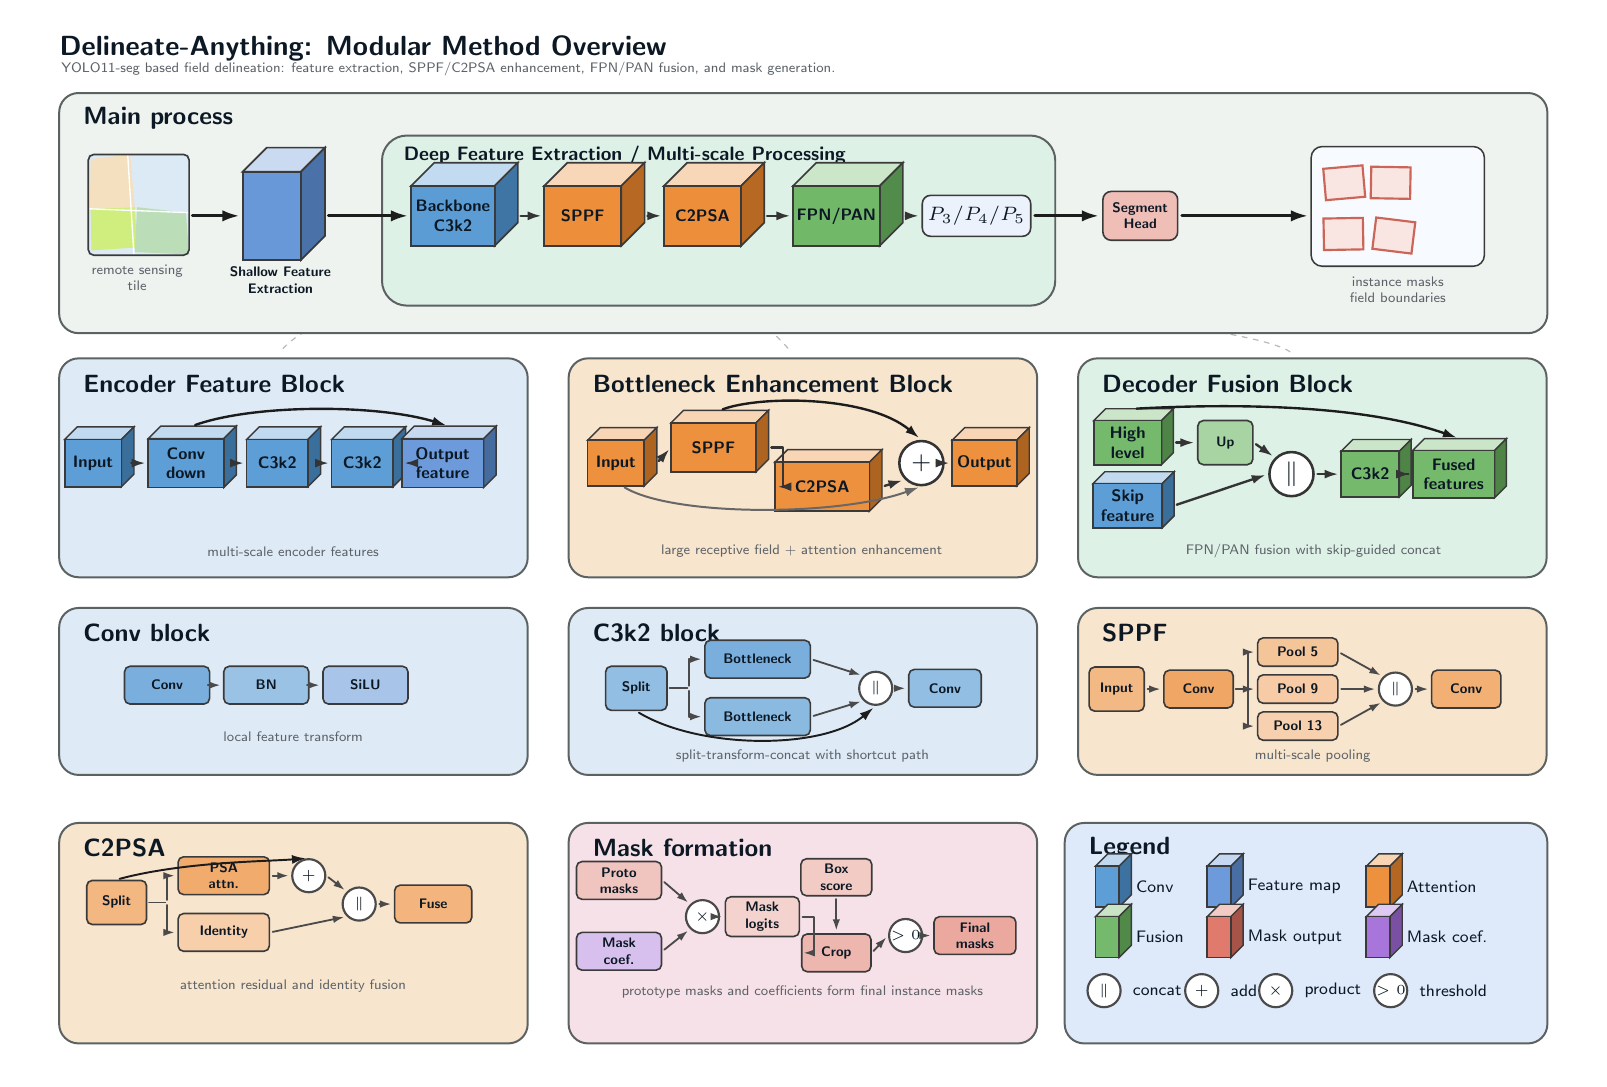
\begin{tikzpicture}[x=1cm,y=1cm]
\path[use as bounding box] (0.15,0.46) rectangle (19.85,13.55);

\node[anchor=west, font=\sffamily\bfseries\fontsize{9.7}{10.8}\selectfont, text=textDark, inner sep=0pt]
  at (0.55,13.28) {Delineate-Anything: Modular Method Overview};
\node[anchor=west, font=\sffamily\fontsize{4.7}{5.5}\selectfont, text=textMuted, inner sep=0pt]
  at (0.57,13.02) {YOLO11-seg based field delineation: feature extraction, SPPF/C2PSA enhancement, FPN/PAN fusion, and mask generation.};

% ---------------------------------------------------------------------
% Main process
% ---------------------------------------------------------------------
\panelbox{0.55}{12.72}{18.90}{3.05}{panelMain}{Main process}

\begin{scope}
  \clip (0.92,10.66) rectangle (2.20,11.94);
  \path[fill=cConv!20] (0.92,10.66) rectangle (2.20,11.94);
  \path[fill=tileFieldA] (0.96,10.72) -- (1.54,10.76) -- (1.51,11.27) -- (0.95,11.25) -- cycle;
  \path[fill=cFusion!45!white] (1.51,10.70) -- (2.20,10.67) -- (2.16,11.20) -- (1.54,11.27) -- cycle;
  \path[fill=tileFieldB] (0.94,11.25) -- (1.51,11.27) -- (1.45,11.94) -- (0.95,11.88) -- cycle;
  \path[draw=white, line width=0.48pt] (1.50,10.66) -- (1.42,11.94);
  \path[draw=white, line width=0.48pt] (0.92,11.25) -- (2.20,11.20);
\end{scope}
\path[draw=lineBlock, line width=0.60pt, rounded corners=2pt] (0.92,10.66) rectangle (2.20,11.94);
\node[note] at (1.54,10.37) {remote sensing\\tile};
\coordinate (tileMainEast) at (2.20,11.16);

\featureblock{topShallow}{3.25}{11.16}{0.74}{1.12}{0.26}{cFeature}{}
\node[note, font=\sffamily\bfseries\tiny, text=textDark] at (3.36,10.34) {Shallow Feature\\Extraction};

\path[panel, fill=panelDecoder, rounded corners=9pt] (4.65,10.02) rectangle (13.20,12.18);
\node[smallTitle] at (4.92,11.92) {Deep Feature Extraction / Multi-scale Processing};

\featureblock{topEnc}{5.55}{11.16}{1.06}{0.76}{0.25}{cConv}{Backbone\\C3k2}
\featureblock{topSppf}{7.20}{11.16}{0.98}{0.76}{0.25}{cAttn}{SPPF}
\featureblock{topC2}{8.72}{11.16}{0.98}{0.76}{0.25}{cAttn}{C2PSA}
\featureblock{topDec}{10.42}{11.16}{1.10}{0.76}{0.25}{cFusion}{FPN/PAN}
\node[flatBlock, fill=panelLegend!60!white, minimum width=1.04cm, minimum height=0.52cm, font=\sffamily\bfseries\scriptsize] (topPyr) at (12.20,11.16) {$P_3/P_4/P_5$};
\draw[coreArrow] (topEnc-east) -- (topSppf-west);
\draw[coreArrow] (topSppf-east) -- (topC2-west);
\draw[coreArrow] (topC2-east) -- (topDec-west);
\draw[coreArrow] (topDec-east) -- (topPyr.west);

\node[flatBlock, fill=cHead!45!white, minimum width=0.95cm, minimum height=0.62cm] (topHead) at (14.28,11.16) {Segment\\Head};
\begin{scope}
  \path[draw=lineBlock, fill=white!75!panelLegend, line width=0.55pt, rounded corners=4pt]
    (16.45,10.52) rectangle (18.65,12.04);
  \foreach \x/\y/\ang in {16.87/11.58/5,17.46/11.58/-1,16.86/10.93/1,17.50/10.91/-7}{
    \path[draw=cHead!92!black, line width=0.78pt, fill=cHead!18, rotate around={\ang:(\x,\y)}]
      ({\x-.25},{\y-.20}) rectangle ({\x+.25},{\y+.20});
  }
  \coordinate (maskDemoWest) at (16.45,11.16);
\end{scope}
\node[note] at (17.55,10.22) {instance masks\\field boundaries};

\draw[mainArrow] (tileMainEast) -- (topShallow-west);
\draw[mainArrow] (topShallow-east) -- (topEnc-west);
\draw[mainArrow] (topPyr.east) -- (topHead.west);
\draw[mainArrow] (topHead.east) -- (maskDemoWest);

% Only three restrained correspondence lines
\begin{scope}[on background layer]
  \draw[mapLine] (topEnc-south) .. controls (4.80,10.10) and (3.65,9.85) .. (3.35,9.42);
  \draw[mapLine] (topC2-south) .. controls (8.92,10.08) and (9.58,9.80) .. (9.85,9.42);
  \draw[mapLine] (topDec-south) .. controls (10.98,10.07) and (15.72,9.82) .. (16.20,9.42);
\end{scope}

% ---------------------------------------------------------------------
% Core module expansion
% ---------------------------------------------------------------------
\panelbox{0.55}{9.35}{5.95}{2.78}{panelEncoder}{Encoder Feature Block}
\panelbox{7.02}{9.35}{5.95}{2.78}{panelBottleneck}{Bottleneck Enhancement Block}
\panelbox{13.49}{9.35}{5.95}{2.78}{panelDecoder}{Decoder Fusion Block}

\slabblock{encIn}{0.98}{8.02}{0.72}{0.60}{0.16}{cConv}{Input}
\slabblock{encDown}{2.16}{8.02}{0.96}{0.62}{0.16}{cConv}{Conv\\down}
\slabblock{encC3a}{3.32}{8.02}{0.78}{0.60}{0.16}{cConv}{C3k2}
\slabblock{encC3b}{4.40}{8.02}{0.78}{0.60}{0.16}{cConv}{C3k2}
\slabblock{encFeat}{5.42}{8.02}{1.04}{0.62}{0.16}{cFeature}{Output\\feature}
\draw[coreArrow] (encIn-east) -- (encDown-west);
\draw[coreArrow] (encDown-east) -- (encC3a-west);
\draw[coreArrow] (encC3a-east) -- (encC3b-west);
\draw[coreArrow] (encC3b-east) -- (encFeat-west);
\draw[shortcut]
  (encDown-north) .. controls (3.02,8.77) and (4.58,8.77) .. (encFeat-north);
\node[note] at (3.52,6.90) {multi-scale encoder features};

\slabblock{botIn}{7.62}{8.02}{0.72}{0.58}{0.16}{cAttn}{Input}
\slabblock{botSppf}{8.86}{8.22}{1.08}{0.62}{0.16}{cAttn}{SPPF}
\slabblock{botPsa}{10.24}{7.72}{1.20}{0.62}{0.16}{cAttn}{C2PSA}
\addnode{botAdd}{11.50}{8.02}
\slabblock{botFeat}{12.30}{8.02}{0.82}{0.58}{0.16}{cAttn}{Output}
\draw[coreArrow] (botIn-east) -- (botSppf-west);
\draw[coreArrow] (botSppf-east) -- ++(0.18,0) |- (botPsa-west);
\draw[coreArrow] (botPsa-east) -- (botAdd.south west);
\draw[coreArrow] (botAdd.east) -- (botFeat-west);
\draw[shortcut]
  (botSppf-north) .. controls (9.46,8.88) and (10.82,8.88) .. (botAdd.north);
\draw[coreArrow, draw=lineCore!75, line width=0.72pt]
  (botIn-south) .. controls (8.34,7.34) and (10.44,7.34) .. (botAdd.south);
\node[note] at (9.98,6.90) {large receptive field + attention enhancement};

\slabblock{decHigh}{14.12}{8.28}{0.86}{0.56}{0.15}{cFusion}{High\\level}
\node[squareBlock, fill=cFusion!58!white, minimum width=0.70cm] (decUp) at (15.36,8.28) {Up};
\slabblock{decSkip}{14.12}{7.48}{0.88}{0.56}{0.15}{cConv}{Skip\\feature}
\concatnode{decConcat}{16.20}{7.88}
\slabblock{decC3}{17.20}{7.88}{0.74}{0.58}{0.15}{cFusion}{C3k2}
\slabblock{decFuse}{18.26}{7.88}{1.04}{0.60}{0.15}{cFusion}{Fused\\features}
\draw[coreArrow] (decHigh-east) -- (decUp.west);
\draw[coreArrow] (decUp.east) -- (decConcat.north west);
\draw[coreArrow] (decSkip-east) -- (decConcat.west);
\draw[coreArrow] (decConcat.east) -- (decC3-west);
\draw[coreArrow] (decC3-east) -- (decFuse-west);
\draw[shortcut]
  (decHigh-north) .. controls (15.50,8.78) and (17.12,8.76) .. (decFuse-north);
\node[note] at (16.48,6.90) {FPN/PAN fusion with skip-guided concat};

% ---------------------------------------------------------------------
% Submodule mechanisms
% ---------------------------------------------------------------------
\panelbox{0.55}{6.18}{5.95}{2.12}{panelEncoder}{Conv block}
\panelbox{7.02}{6.18}{5.95}{2.12}{panelEncoder}{C3k2 block}
\panelbox{13.49}{6.18}{5.95}{2.12}{panelBottleneck}{SPPF}

\node[flatLong, fill=cConv!76!white, minimum width=1.08cm] (convA) at (1.92,5.20) {Conv};
\node[flatLong, fill=cConv!58!white, minimum width=1.08cm] (convB) at (3.18,5.20) {BN};
\node[flatLong, fill=cFeature!54!white, minimum width=1.08cm] (convC) at (4.44,5.20) {SiLU};
\draw[subArrow] (convA.east) -- (convB.west);
\draw[subArrow] (convB.east) -- (convC.west);
\node[note] at (3.52,4.55) {local feature transform};

\node[squareBlock, fill=cConv!62!white, minimum width=0.78cm] (c3Split) at (7.88,5.16) {Split};
\node[flatLong, fill=cConv!76!white, minimum width=1.34cm] (c3B1) at (9.42,5.53) {Bottleneck};
\node[flatLong, fill=cConv!66!white, minimum width=1.34cm] (c3B2) at (9.42,4.80) {Bottleneck};
\smallconcat{c3Cat}{10.92}{5.16}
\node[flatLong, fill=cConv!62!white, minimum width=0.92cm] (c3Conv) at (11.80,5.16) {Conv};
\coordinate (c3Fork) at (8.55,5.16);
\draw[branchLine] (c3Split.east) -- (c3Fork);
\draw[subArrow] (c3Fork) |- (c3B1.west);
\draw[subArrow] (c3Fork) |- (c3B2.west);
\draw[subArrow] (c3B1.east) -- (c3Cat.north west);
\draw[subArrow] (c3B2.east) -- (c3Cat.south west);
\draw[subArrow] (c3Cat.east) -- (c3Conv.west);
\draw[shortcut, line width=0.70pt]
  (c3Split.south) .. controls (8.70,4.38) and (10.25,4.38) .. (c3Cat.south);
\node[note] at (9.99,4.30) {split-transform-concat with shortcut path};

\node[squareBlock, fill=cAttn!58!white, minimum width=0.70cm] (sppfIn) at (13.98,5.15) {Input};
\node[flatLong, fill=cAttn!74!white, minimum width=0.88cm] (sppfConv1) at (15.02,5.15) {Conv};
\node[flatLong, fill=cAttn!48!white, minimum width=1.02cm, minimum height=0.36cm] (poolA) at (16.28,5.62) {Pool 5};
\node[flatLong, fill=cAttn!43!white, minimum width=1.02cm, minimum height=0.36cm] (poolB) at (16.28,5.15) {Pool 9};
\node[flatLong, fill=cAttn!38!white, minimum width=1.02cm, minimum height=0.36cm] (poolC) at (16.28,4.68) {Pool 13};
\smallconcat{sppfJoin}{17.52}{5.15}
\node[flatLong, fill=cAttn!66!white, minimum width=0.88cm] (sppfConv2) at (18.42,5.15) {Conv};
\draw[subArrow] (sppfIn.east) -- (sppfConv1.west);
\coordinate (poolStem) at (15.65,5.15);
\draw[branchLine] (sppfConv1.east) -- (poolStem);
\draw[lineSub, line width=0.62pt, line cap=round] (poolStem) -- (15.65,5.62);
\draw[lineSub, line width=0.62pt, line cap=round] (poolStem) -- (15.65,4.68);
\draw[subArrow] (15.65,5.62) -- (poolA.west);
\draw[subArrow] (poolStem) -- (poolB.west);
\draw[subArrow] (15.65,4.68) -- (poolC.west);
\draw[subArrow] (poolA.east) -- (sppfJoin.north west);
\draw[subArrow] (poolB.east) -- (sppfJoin.west);
\draw[subArrow] (poolC.east) -- (sppfJoin.south west);
\draw[subArrow] (sppfJoin.east) -- (sppfConv2.west);
\node[note] at (16.47,4.30) {multi-scale pooling};

\panelbox{0.55}{3.45}{5.95}{2.80}{panelBottleneck}{C2PSA}
\panelbox{7.02}{3.45}{5.95}{2.80}{panelMask}{Mask formation}
\panelbox{13.32}{3.45}{6.13}{2.80}{panelLegend}{Legend}

\begin{scope}[yshift=-0.44cm]

\node[squareBlock, fill=cAttn!60!white, minimum width=0.76cm] (c2Split) at (1.28,2.88) {Split};
\node[flatLong, fill=cAttn!70!white, minimum width=1.16cm] (c2Psa) at (2.64,3.22) {PSA\\attn.};
\smalladd{c2Add}{3.72}{3.22}
\node[flatLong, fill=cAttn!40!white, minimum width=1.16cm] (c2Id) at (2.64,2.50) {Identity};
\smallconcat{c2Join}{4.36}{2.86}
\node[flatLong, fill=cAttn!62!white, minimum width=0.98cm] (c2Fuse) at (5.30,2.86) {Fuse};
\coordinate (c2Fork) at (1.92,2.88);
\draw[branchLine] (c2Split.east) -- (c2Fork);
\draw[subArrow] (c2Fork) |- (c2Psa.west);
\draw[subArrow] (c2Fork) |- (c2Id.west);
\draw[subArrow] (c2Psa.east) -- (c2Add.west);
\draw[subArrow] (c2Add.east) -- (c2Join.north west);
\draw[subArrow] (c2Id.east) -- (c2Join.south west);
\draw[subArrow] (c2Join.east) -- (c2Fuse.west);
\draw[shortcut, line width=0.70pt]
  (c2Split.north) .. controls (2.15,3.40) and (3.18,3.40) .. (c2Add.north);
\node[note] at (3.52,1.82) {attention residual and identity fusion};

\node[flatLong, fill=cHead!40!white, minimum width=1.08cm] (proto) at (7.66,3.16) {Proto\\masks};
\node[flatLong, fill=cMask!42!white, minimum width=1.08cm] (coef) at (7.66,2.26) {Mask\\coef.};
\smallproduct{maskMul}{8.72}{2.70}
\node[flatLong, fill=cHead!30!white, minimum width=0.94cm] (logits) at (9.48,2.70) {Mask\\logits};
\node[flatLong, fill=cHead!36!white, minimum width=0.90cm, minimum height=0.40cm] (box) at (10.42,3.20) {Box\\score};
\node[flatLong, fill=cHead!50!white, minimum width=0.88cm] (crop) at (10.42,2.24) {Crop};
\smallthreshold{thr}{11.30}{2.46}
\node[flatLong, fill=cHead!60!white, minimum width=1.04cm] (finalMask) at (12.18,2.46) {Final\\masks};
\draw[subArrow] (proto.east) -- (maskMul.north west);
\draw[subArrow] (coef.east) -- (maskMul.south west);
\draw[subArrow] (maskMul.east) -- (logits.west);
\draw[subArrow] (logits.east) -- ++(0.18,0) |- (crop.west);
\draw[subArrow] (box.south) -- (crop.north);
\draw[subArrow] (crop.east) -- (thr.west);
\draw[subArrow] (thr.east) -- (finalMask.west);
\node[note] at (9.99,1.74) {prototype masks and coefficients form final instance masks};

\subblock{lgConv}{13.86}{3.08}{0.30}{0.52}{0.14}{cConv}{}
\node[legendText] at (14.22,3.08) {Conv};
\subblock{lgFeat}{15.28}{3.08}{0.30}{0.52}{0.14}{cFeature}{}
\node[legendText] at (15.64,3.08) {Feature map};
\subblock{lgAttn}{17.30}{3.08}{0.30}{0.52}{0.14}{cAttn}{}
\node[legendText] at (17.66,3.08) {Attention};

\subblock{lgFuse}{13.86}{2.44}{0.30}{0.52}{0.14}{cFusion}{}
\node[legendText] at (14.22,2.44) {Fusion};
\subblock{lgHead}{15.28}{2.44}{0.30}{0.52}{0.14}{cHead}{}
\node[legendText] at (15.64,2.44) {Mask output};
\subblock{lgAux}{17.30}{2.44}{0.30}{0.52}{0.14}{cMask}{}
\node[legendText] at (17.66,2.44) {Mask coef.};

\smallconcat{lgCat}{13.82}{1.76}
\node[legendText] at (14.18,1.76) {concat};
\smalladd{lgAdd}{15.06}{1.76}
\node[legendText] at (15.42,1.76) {add};
\smallproduct{lgProd}{16.00}{1.76}
\node[legendText] at (16.36,1.76) {product};
\smallthreshold{lgThr}{17.46}{1.76}
\node[legendText] at (17.82,1.76) {threshold};

\end{scope}

\end{tikzpicture}
\end{document}
